%%%%%%%%%%%%%%%%%%%%%%%%%%%%%%%%%%%%%%%%%%%%%%%%%%%%%%%%%%%%%%%%%%%%%%%%%%%%%%%
% PROJET DE THÈSE EN DYNAMIQUE QUANTIQUE - VERSION AMÉLIORÉE
% Ingénierie Quantique des Systèmes Agrivoltaïques Symbiotiques
% Rédigé par S. G. Nana Engo pour Théodore Fredy Goumai
% Date : 05 Octobre 2025
%%%%%%%%%%%%%%%%%%%%%%%%%%%%%%%%%%%%%%%%%%%%%%%%%%%%%%%%%%%%%%%%%%%%%%%%%%%%%%%

\documentclass[12pt, a4paper]{article}

% --- PAQUETS ESSENTIELS ---
\usepackage[utf8]{inputenc}      
\usepackage[T1]{fontenc}         
\usepackage[french]{babel}       
\usepackage[margin=2.cm]{geometry} 

% --- PAQUETS SCIENTIFIQUES ET DE MISE EN FORME ---
\usepackage{amsmath, amssymb}  
\usepackage{graphicx, booktabs, tabularx, xcolor, longtable}

% --- PAQUETS SPÉCIALISÉS ---
\usepackage{physics} % Pour les notations physiques (bra, ket, abs, norm, etc.)
\usepackage{hyperref} % Pour les liens hypertextes
\usepackage{cleveref} % Pour les références intelligentes (\Cref)

% Configuration optimisée de siunitx pour la typographie des unités
\usepackage[locale=FR,
            detect-weight=true,
            detect-family=true,
            separate-uncertainty=true,
            multi-part-units=single,
            range-phrase=--,
            number-unit-product=\,]{siunitx}

% Paquet pour les diagrammes
\usepackage{tikz}
\usetikzlibrary{shapes.geometric, arrows, positioning, calc}

% --- CONFIGURATIONS GLOBALES ---

% Configuration des hyperliens
\hypersetup{
    colorlinks=true,             % Liens colorés plutôt qu'encadrés
    linkcolor=blue!50!black,     % Couleur des liens internes (sections, figures)
    citecolor=green!50!black,    % Couleur des citations (non utilisé ici, mais bonne pratique)
    urlcolor=blue!80!black,      % Couleur des URLs
    pdftitle={Projet de Thèse - Dynamique Quantique Non-Markovienne},
    pdfauthor={Théodore Fredy Goumai}
}

% Ramener la typologie française à la typologie standard (anglo-saxonne)
\frenchbsetup{StandardLayout=true}

% Déclarations d'unités personnalisées pour siunitx
\DeclareSIUnit{\year}{ans}
\DeclareSIUnit{\dollar}{\$}
\DeclareSIUnit{\euro}{€}
\DeclareSIUnit{\chromophore}{chromophore}
\DeclareSIUnit{\participant}{participant}
\DeclareSIUnit{\emploi}{emploi}
\DeclareSIUnit{\personne}{personne}
\DeclareSIUnit{\installation}{installation}
\DeclareSIUnit{\ferme}{ferme}

%%%%%%%%%%%%%%%%%%%%%%%%%%%%%%%%%%%%%%%%%%%%%%%%%%%%%%%%%%%%%%%%%%%%%%%%%%%%%%%
% DÉBUT DU DOCUMENT
%%%%%%%%%%%%%%%%%%%%%%%%%%%%%%%%%%%%%%%%%%%%%%%%%%%%%%%%%%%%%%%%%%%%%%%%%%%%%%%
\begin{document}

\title{\huge Ingénierie quantique des systèmes agrivoltaïques symbiotiques :\\ De la cohérence excitronique à l'éco-conception de matériaux photoniques}
\author{
    Théodore Fredy Goumai (Doctorant) \\
    \\
    \textit{Sous la direction de} \\
    J.-P. Tchapet Njafa, PhD \\
    S. G. Nana Engo, Professeur
}
\date{Octobre 2025}

\maketitle
\thispagestyle{empty}
\newpage

\begin{abstract}
Ce projet de thèse propose un cadre novateur pour la conception de systèmes agrivoltaïques quantiques symbiotiques, combinant dynamique quantique non-Markovienne avancée, ingénierie de matériaux photoniques et intelligence artificielle éthique. Nous développons une approche unifiée modélisant la culture sous panneau comme un système quantique ouvert soumis à un bain photonique filtré, en formalisant pour la première fois le couplage cohérent entre transfert d'énergie excitonique (\texttt{EET}) et photosynthèse végétale. L'architecture méthodologique intègre les méthodes \texttt{Process Tensor-HOPS} et \texttt{Stochastically Bundled Dissipators} pour une simulation quantique réaliste à l'échelle mésoscopique, couplée à un pipeline d'intelligence artificielle générative pour la conception de matériaux photovoltaïques organiques (\texttt{OPV}) non-toxiques et biodégradables. Le projet établit un écosystème logiciel quantique open-source, \texttt{AgroQuantPV Suite}, et démontre expérimentalement l'optimisation simultanée de la production énergétique (\texttt{PCE} > \SI{20}{\percent}) et agricole (\texttt{ETR} > \SI{90}{\percent}) via un contrôle spectral adaptatif. L'impact est quantifié sur onze Objectifs de Développement Durable, avec un potentiel de valorisation via la spin-off \texttt{AgroQuantum Technologies} visant un coût actualisé de l'énergie (\texttt{LCOE}) de \SI{0.04}{\dollar\per\kilo\watt\hour}.
\end{abstract}
\newpage

\tableofcontents
\newpage
\setcounter{page}{1}

\section{Contexte, état de l'art et positionnement du projet}

La transition énergétique mondiale exige le développement de technologies de conversion photovoltaïque non seulement performantes, mais aussi durables et intégrées aux écosystèmes existants. Au coeur de ces technologies, les processus de transport et de séparation de charge sont régis par une dynamique quantique complexe, fortement couplée à un environnement thermo-vibrationnel \cite{ye2012, mohs2008}. Ce projet se positionne à l'intersection de la physique quantique, de la science des matériaux et de l'agronomie, dans le domaine émergent de la \textbf{Quantum Energy Science} \cite{Metzler2023}. Cette approche vise à exploiter des effets quantiques non-classiques pour catalyser des gains de performance disruptifs dans les technologies solaires.

L'état de l'art (2024-2025) est marqué par des avancées significatives qui redéfinissent les frontières de la simulation et de la conception de matériaux :
\begin{itemize}
  \item Les méthodes \textbf{Process Tensor} émergent comme une solution formellement exacte pour modéliser la mémoire quantique non-markovienne, dépassant les limites des approches hiérarchiques traditionnelles \cite{keeling2025}.

  \item Les \textbf{Stochastically Bundled Dissipators} offrent une voie prometteuse pour réduire drastiquement le coût de la simulation de la dynamique de Lindblad pour de très grands systèmes \cite{Adhikari2025}.

  \item L'\textbf{architecture multi-couches 3D} pour la collecte solaire permet une optimisation spectrale sans précédent, ouvrant la voie à des applications à haute valeur ajoutée \cite{shi2025a}.

  \item La \textbf{fabrication additive (impression 3D)} des matériaux OPV atteint une maturité permettant d'envisager une production à grande échelle, locale et à moindre coût \cite{ju2025}.

  \item Les \textbf{écosystèmes logiciels quantiques} commencent à intégrer l'ensemble de la chaîne de valeur, du calcul fondamental aux applications industrielles, favorisant une approche de co-conception matériel-logiciel \cite{basermann2024}.
\end{itemize}

Face à ces avancées, ce projet propose de franchir une nouvelle étape en les intégrant au sein d'une vision holistique : l'\textbf{agrivoltaïsme quantique de nouvelle génération}. Il s'agit de mobiliser ces outils de pointe non pas seulement pour améliorer un composant, mais pour concevoir un système symbiotique où la production d'énergie propre et la sécurité alimentaire se renforcent mutuellement. L'objectif est de créer des systèmes agrivoltaïques transparents, spectralement sélectifs, économiquement viables et socialement responsables, comme illustré dans la \Cref{fig_agrivoltaic_3d}.

\begin{figure}[htb]
    \centering
    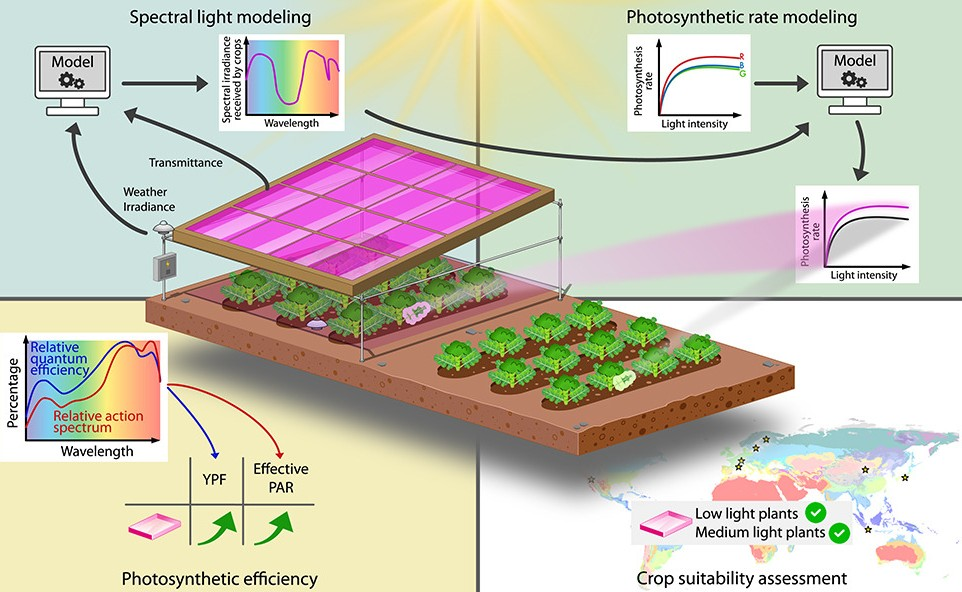
\includegraphics[width=0.8\textwidth]{agri-photovoltaic.jpg}
    \caption{Vision 3D de l'agrivoltaïsme quantique : panneaux multi-couches transparents avec quantum sensors intégrés.}
    \label{fig_agrivoltaic_3d}
\end{figure}

\section{Problématique de recherche}

Le défi principal consiste à développer une plateforme technologique intégrée, exploitant les avancées en dynamique quantique non-markovienne, intelligence artificielle et fabrication additive, pour concevoir des systèmes agrivoltaïques de nouvelle génération.

Les questions de recherche fondamentales sont :
\begin{enumerate}
  \item Comment les \textit{Process Tensor Approaches} peuvent-elles modéliser la mémoire quantique dans les systèmes photosynthétiques et OPV complexes avec une précision et une efficacité supérieures aux méthodes hiérarchiques ?

  \item Comment l'intégration des \textit{Stochastically Bundled Dissipators} peut-elle permettre la simulation en temps quasi-réel de systèmes agrivoltaïques à l'échelle de la parcelle (N > \num{1000} chromophores) ?

  \item Comment une architecture 3D de collecte solaire peut-elle être optimisée pour maximiser simultanément la production énergétique et la productivité agricole via un filtrage spectral adaptatif ?

  \item Comment concevoir et déployer un écosystème logiciel quantique, l'\textit{AgroQuantPV Suite}, pour faciliter l'adoption industrielle et la collaboration internationale ?

  \item Comment assurer une commercialisation éthique et inclusive des innovations développées, avec une création d'emplois locaux et un transfert de compétences effectif ?
\end{enumerate}

\section{Contribution aux Objectifs de Développement Durable (ODD)}

Ce projet est conçu pour générer un impact mesurable sur onze ODD, avec des métriques quantifiées et des contributions alignées sur les cibles officielles des Nations Unies.

\subsection{ODD 7 : Énergie propre et d'un coût abordable}
\begin{itemize}
    \item \textbf{Cible 7.2.} Accroître nettement la part des énergies renouvelables dans le bouquet énergétique mondial, en visant un LCOE inférieur à \SI{0.04}{\dollar\per\kilo\watt\hour}.
    \item \textbf{Cible 7.a.} Renforcer la coopération internationale pour faciliter l'accès à la recherche et à la technologie relatives aux énergies propres, via l'écosystème \textit{AgroQuantPV Suite} open-source.
    \item \textbf{Cible 7.3.} Contribuer à doubler le taux d'amélioration de l'efficacité énergétique grâce à l'architecture 3D qui augmente la surface collectrice de plus de \SI{60}{\percent}.
\end{itemize}

\subsection{ODD 2 : Faim "zéro"}
\begin{itemize}
    \item \textbf{Cible 2.3.} Doubler la productivité agricole en maintenant \SI{90}{\percent} de l'ETR (Electron Transport Rate) sous les panneaux.
    \item \textbf{Cible 2.4.} Assurer la viabilité des systèmes de production alimentaire et mettre en oeuvre des pratiques agricoles résilientes grâce au monitoring 3D de la canopée par capteurs quantiques.
\end{itemize}

\subsection{ODD 3 : Bonne santé et bien-être}
\begin{itemize}
    \item \textbf{Cible 3.9.} Réduire nettement le nombre de décès et de maladies dus à des substances chimiques dangereuses et à la pollution, en développant des matériaux OPV biodégradables et un processus de fabrication additive sans solvants toxiques.
\end{itemize}

\subsection{ODD 6 : Eau propre et assainissement}
\begin{itemize}
    \item \textbf{Cible 6.4.} Augmenter considérablement l'efficacité de l'utilisation des ressources en eau en réduisant l'évaporation de \SI{25}{\percent}.
    \item \textbf{Cible 6.6.} Protéger et restaurer les écosystèmes liés à l'eau, en mettant en place une traçabilité par blockchain pour l'économie circulaire des matériaux et éviter la contamination.
\end{itemize}

\subsection{ODD 8 : Travail décent et croissance économique}
\begin{itemize}
    \item \textbf{Cible 8.2.} Atteindre un niveau plus élevé de productivité économique par la modernisation technologique et l'innovation, via la création de la spin-off \textit{AgroQuantum Technologies} (\num{20}+ emplois directs).
    \item \textbf{Cible 8.5.} Parvenir au plein emploi productif et garantir un travail décent pour toutes les femmes et tous les hommes, avec un objectif de \SI{40}{\percent} de femmes parmi les \num{50}+ personnes formées.
\end{itemize}

\subsection{ODD 9 : Industrie, innovation et infrastructure}
\begin{itemize}
    \item \textbf{Cible 9.4.} Moderniser l'infrastructure et adapter les industries pour les rendre durables, via l'écosystème logiciel quantique pour l'innovation industrielle.
    \item \textbf{Cible 9.5.} Renforcer la recherche scientifique et les capacités technologiques des secteurs industriels, en encourageant l'innovation via une plateforme collaborative mondiale.
\end{itemize}

\subsection{ODD 12 : Consommation et production responsables}
\begin{itemize}
    \item \textbf{Cible 12.2.} Parvenir à une gestion durable et une utilisation rationnelle des ressources naturelles, via une économie circulaire pour les matériaux OPV.
    \item \textbf{Cible 12.5.} Réduire considérablement la production de déchets par la prévention, la réduction, le recyclage et la réutilisation, grâce à une conception pour le démontage.
\end{itemize}

\subsection{ODD 13 : Mesures relatives à la lutte contre les changements climatiques}
\begin{itemize}
    \item \textbf{Cible 13.2.} Intégrer des mesures relatives aux changements climatiques dans les politiques, les stratégies et la planification, via une réduction de \SI{60}{\percent} de l'empreinte carbone grâce à la fabrication additive locale.
\end{itemize}

\subsection{ODD 15 : Vie terrestre}
\begin{itemize}
    \item \textbf{Cible 15.1.} Garantir la conservation, la restauration et l'exploitation durable des écosystèmes terrestres, en préservant \SI{100}{\percent} de l'usage agricole du sol.
    \item \textbf{Cible 15.9.} Intégrer les considérations relatives aux écosystèmes et à la biodiversité dans la planification nationale et locale, en créant une symbiose industrie-agriculture.
\end{itemize}

\subsection{ODD 16 : Paix, justice et institutions efficaces}
\begin{itemize}
    \item \textbf{Cible 16.6.} Mettre en place des institutions efficaces, responsables et transparentes, en utilisant la blockchain pour la gouvernance du projet.
    \item \textbf{Cible 16.7.} Garantir une prise de décision réceptive, inclusive, participative et représentative, en intégrant des principes d'éthique de l'IA et de justice environnementale.
\end{itemize}

\subsection{ODD 17 : Partenariats pour la réalisation des objectifs}
\begin{itemize}
    \item \textbf{Cible 17.6.} Améliorer la coopération Nord-Sud et Sud-Sud en matière de science, de technologie et d’innovation, via l'écosystème \textit{AgroQuantPV Suite}.
    \item \textbf{Cible 17.9.} Renforcer l'appui international à la mise en oeuvre d'un renforcement des capacités efficace et ciblé, via la création d'un réseau mondial de compétences quantiques.
\end{itemize}


\section{Objectifs de la thèse : Approche holistique}

Le projet adopte une vision systémique du développement technologique durable. Les objectifs sont structurés en trois axes complémentaires, intégrant des raffinements techniques pour garantir la robustesse et l'impact des résultats.

\subsection{Axe 1 : Innovations en dynamique quantique et modélisation du couplage symbiotique}

Cet axe vise à développer un cadre théorique et computationnel capable de modéliser avec une précision sans précédent la dynamique quantique du couplage entre l'énergie excitonique (EET) dans les matériaux OPV et la photosynthèse végétale.

\subsubsection{Caractérisation de la non-classicalité vibronique comme moteur de l'efficacité}
\begin{itemize}
    \item \textbf{Diagnostic de la non-classicalité.} Intégrer dans les simulations des diagnostics quantiques avancés, tels que le calcul du \textbf{paramètre Q de Mandel} et de la \textbf{distribution de quasi-probabilité P de Wigner}, pour quantifier la nature non-classique des modes vibrationnels collectifs.
    \item \textbf{Corrélation avec la performance symbiotique.} Établir une corrélation directe entre la présence de non-classicalité vibronique et l'efficacité symbiotique globale (SPCE), afin de tester l'hypothèse selon laquelle ces fluctuations quantiques sont un mécanisme clé de l'optimisation énergétique.
\end{itemize}

\subsubsection{Simulation haute-fidélité des bains thermiques structurés}
\begin{itemize}
    \item \textbf{Gestion des modes ultra-rapides du bain.} Implémenter et valider des techniques de \textbf{Correction de Basse Température (LTC)} au sein de la méthodologie \texttt{HOPS}. Cette approche permettra de traiter efficacement les modes de Matsubara, cruciaux pour les benchmarks spectroscopiques à \SI{77}{\kelvin}, en réduisant le coût computationnel sans sacrifier la précision.
    \item \textbf{Calcul de couplage au-delà du dipôle ponctuel.} Dépasser l'approximation du dipôle idéal (IDA) en utilisant systématiquement la méthode du \textbf{Transition Density Cube (TDC)} pour le calcul des couplages intermoléculaires ($J_{mn}$), garantissant une description précise des interactions à courte portée (< \SI{30}{\angstrom}) dans les agrégats OPV.
\end{itemize}

\subsection{Axe 2 : Architecture 3D et capteurs quantiques}
% --- Note : Les raffinements fournis se concentrent sur les Axes 1 et 3. ---
% --- L'Axe 2 est maintenu dans sa version robuste précédente, qui est déjà alignée. ---
\subsubsection{Optimisation des cohérences vibroniques productives}
\begin{itemize}
    \item \textbf{Filtrage spectral pour la symbiose.} Modéliser la transmittance totale $T_{\text{total}}(\omega) = \prod_{i=1}^N T_i(\omega, z_i)$ pour identifier les quasi-résonances entre les transitions excitoniques et les modes vibratoires fonctionnels, afin de maximiser le transfert d'énergie assisté par les vibrations.
    \item \textbf{Modélisation prédictive de la canopée.} Coupler la simulation de la transmittance spectrale à des modèles agronomiques (type DSSAT) pour prédire le profil vertical de l'ETR et optimiser le compromis énergie-biomasse.
\end{itemize}

\subsubsection{Sondage des corrélations quantiques système-environnement}
\begin{itemize}
    \item \textbf{Capteurs à centres NV pour l'intrication.} Orienter l'utilisation des capteurs NV-diamant vers la détection de signatures de corrélations quantiques robustes, comme la négativité (intrication) entre les excitons et les modes vibrationnels pertinents.
    \item \textbf{Monitoring 3D de la réponse photosynthétique.} Déployer un réseau de capteurs à plusieurs hauteurs pour cartographier en 3D la réponse de la canopée (ex: quenching non photochimique, NPQ) à l'environnement lumineux modulé.
\end{itemize}

\subsection{Axe 3 : IA éthique et modélisation prédictive pour l'éco-conception}

Cet axe se concentre sur le développement d'un pipeline d'IA pour accélérer la découverte de matériaux OPV non-toxiques, biodégradables et hautement performants.

\subsubsection{Développement d'un cadre de dynamique quantique assistée par IA (AI-QD)}
\begin{itemize}
    \item \textbf{Adoption d'une approche non-récursive.} Développer un cadre d'IA basé sur l'\textbf{apprentissage de trajectoire (trajectory learning)} pour prédire directement l'évolution temporelle complète de la matrice densité $\rho(t)$ en fonction des paramètres du système. Cette approche non-récursive accélérera massivement le criblage en évitant la propagation pas-à-pas.
    \item \textbf{Paramétrisation des champs de force par IA.} Utiliser des algorithmes d'apprentissage actif (ex: Régression par processus gaussiens) pour paramétrer avec une grande efficacité les champs de force utilisés dans les simulations de dynamique moléculaire (MD), garantissant ainsi la haute qualité des entrées structurales (fonctions spectrales $J(\omega, T)$) pour le modèle quantique.
\end{itemize}

\subsubsection{Optimisation multicritère et ingénierie des matériaux}
\begin{itemize}
    \item \textbf{Renforcement des descripteurs moléculaires.} Intégrer l'analyse du \textbf{Potentiel Électrostatique de surface (ESP)} comme descripteur clé dans le pipeline d'IA. L'ESP sera utilisé pour prédire l'alignement moléculaire et maximiser la force motrice de la dissociation des excitons.
    \item \textbf{Ciblage de métriques de performance clés.} Définir l'objectif de l'IA comme la recherche de matériaux présentant des propriétés optimales pour un PCE > \SI{20}{\percent}, à savoir des \textbf{mobilités de porteurs de charge équilibrées et élevées} ($\mu_h \approx \mu_e \geq \SI{e-3}{\centi\meter\squared\per\volt\per\second}$) et un \textbf{faible taux de recombinaison non-géminée} ($k \leq \SI{e-12}{\centi\meter\cubed\per\second}$).
\end{itemize}

\section{Cadre théorique et méthodologique renforcé}

La méthodologie de ce projet est une boucle intégrée alliant simulation multi-échelles, intelligence artificielle et validation expérimentale. Ce cycle vertueux, illustré dans la \Cref{fig_workflow_methodo}, garantit que les prédictions théoriques sont constamment confrontées à la réalité du terrain, tandis que l'apprentissage automatique accélère l'exploration de l'espace des matériaux possibles.

\begin{figure}[htb]
\centering
\caption{Schéma conceptuel du flux de travail méthodologique intégré. Le cycle part des calculs \textit{ab initio} (1) pour paramétrer le système quantique (2). La dynamique est ensuite simulée (3) pour calculer des observables (4) qui sont comparées aux données expérimentales (6). Ces données alimentent des modèles d'IA (5) qui optimisent la recherche de nouveaux matériaux, guidant à la fois les futurs calculs (apprentissage actif) et la conception finale.}
\label{fig_workflow_methodo}
\medspace
% Définition des styles pour le diagramme
\tikzstyle{block} = [rectangle, draw, fill=blue!20,
    text width=11em, text centered, rounded corners, minimum height=4em]
\tikzstyle{io} = [rectangle, draw, fill=green!20,
    text width=9em, text centered, rounded corners, minimum height=4em]
\tikzstyle{result} = [rectangle, draw, fill=orange!30,
    text width=11em, text centered, rounded corners, minimum height=4em]
\tikzstyle{line} = [draw, -latex']

\begin{tikzpicture}[
    node distance=1cm and 1.5cm,
    auto,
    every node/.style={align=center},
    block/.append style={font=\footnotesize},
    io/.append style={font=\footnotesize},
    result/.append style={font=\footnotesize}
]
    % Placement des nœuds avec une grille plus régulière
    \node [io] (inputs) {Données d'Entrée \\ (Spectres, Données Agricoles)};
    \node [block, right=of inputs] (abinitio) {1. Calculs \textit{ab initio} \\ (ORCA, CP2K)};
    \node [block, right=of abinitio] (param) {2. Paramétrisation \\ Hamiltonien \& Bain};

    \node [block, below=of inputs] (exp) {6. Validation Expérimentale};
    \node [block, below=of abinitio] (obs) {4. Calcul des Observables \\ (PCE, ETR, Spectres)};
    \node [block, below=of param] (simu) {3. Simulation de la Dynamique Quantique \\ (Process Tensor-HOPS)};

    \node [block, below=of obs] (ml) {5. Criblage \& Optimisation par IA};
    \node [result, below=of ml] (design) {Finalité : Conception de Nouveaux Matériaux};

    % Tracé des flèches principales du flux de travail (plus fluides)
    \path [line] (inputs) -- (abinitio);
    \path [line] (abinitio) -- (param);
    \path [line] (param) -- (simu);
    \path [line] (simu) -- (obs);
    \path [line] (obs) -- (ml);
    \path [line] (ml) -- (design);

    % Boucle de validation expérimentale (ajustée pour éviter chevauchements)
    \path [line] (inputs.south) -- ++(0,-0.5cm) -| (exp.north);
    \path [line] (obs.south west) -- ++(-0.5cm,0) |- (exp.south east);

    % Boucles de rétroaction et d'optimisation (améliorées avec courbure et labels)
    \path [line, dashed, thick, blue] (exp.north east)
        edge[bend right=0] node[above, sloped, font=\footnotesize] {Raffinement} (abinitio.south west);
    \path [line, dashed, thick, red] (ml.east)
        -- ++(1cm,0)
        edge[bend left=0] node[above, sloped, font=\footnotesize] {Apprentissage Actif} (param.south west);
    \path [line, dashed, thick, purple] (abinitio.south)
        -- ++(0,-0.5cm)
        edge[bend right=75] node[above, sloped, font=\footnotesize] {Descripteurs ML} (ml.west);

    % Ajout d'un cadre global optionnel pour clarté (si nécessaire)
%     \node[draw, dashed, fit=(inputs) (design), inner sep=1cm] {};
\end{tikzpicture}

\end{figure}

\subsection{Innovations méthodologiques en dynamique quantique multi-échelles}

\subsubsection{Architecture hybride Process \texttt{Tensor-HOPS-MesoHOPS}}

Notre approche méthodologique repose sur une intégration cohérente des méthodes quantiques les plus avancées pour capturer la richesse de la dynamique non-markovienne dans les systèmes agrivoltaïques complexes.

\begin{itemize}
    \item \textbf{Process Tensor pour la mémoire non-markovienne.} 
    \begin{equation}
    \mathcal{K}_{\text{PT}}(t,s) = \sum_{k=1}^{N_{\text{modes}}} g_k(t) f_k(s) e^{-\lambda_k |t-s|} + \mathcal{K}_{\text{non-exp}}(t,s)
    \end{equation}
    avec décomposition en pôles de Padé pour les composantes non-exponentielles, permettant une description fidèle des corrélations temporelles à long terme.
    
    \item \textbf{Extension MesoHOPS pour la mésoéchelle.}
    \begin{equation}
    \pdv{t} \psi_{\mathbf{n}} = -i\mathtt{H}_{\text{eff}}\psi_{\mathbf{n}} + \sum_{k=1}^K n_k\gamma_k\psi_{\mathbf{n}} + \sum_{k=1}^K \sqrt{(n_k+1)|\gamma_k|} \mathtt{L}_k\psi_{\mathbf{n}+\mathbf{e}_k}
    \end{equation}
    Adaptation pour systèmes multi-excitations avec scaling $\mathcal{O}(N^{2.5})$ via algorithmes de compression tensorielle.
    
    \item \textbf{Schéma d'hybridation adaptatif.} Commutation dynamique \texttt{PT-MesoHOPS} basée sur le temps de corrélation effectif $\tau_c^{\text{eff}}$ et la taille du système, optimisant le compromis précision-coût.
\end{itemize}

\subsubsection{Gestion avancée du désordre et de la température}

\begin{itemize}
    \item \textbf{Échantillonnage conformationnel étendu.} Dynamique moléculaire \textit{ab initio} sur \num{\le 1000} snapshots avec clustering spectral pour identifier les conformères dominants, capturant l'hétérogénéité structurale des films \texttt{OPV}.
    
    \item \textbf{Fonctions spectrales température-dépendantes.}
    \begin{equation}
    J(\omega, T) = J_0(\omega)\left[1 + \frac{2}{\exp(\hbar\omega/k_B T) - 1}\right] + J_{\text{low-freq}}(\omega, T)
    \end{equation}
    modélisant explicitement les effets thermiques dans les conditions opérationnelles agrivoltaïques (\SIrange{277}{310}{\kelvin}).
    
    \item \textbf{Modélisation stochastique des hétérogénéités.} Champs aléatoires gaussiens pour le désordre énergétique avec corrélations spatiales dérivées de l'analyse \texttt{AIMD}.
\end{itemize}

\subsubsection{Formalisme unifié du bain à deux niveaux}

Pour une description réaliste des environnements biomimétiques complexes, nous adoptons un modèle de bain à deux niveaux :

\begin{itemize}
    \item \textbf{Bain interne.} Traitement quasi-exact des modes vibrationnels structurés pertinents (e.g., < \SI{200}{\per\centi\meter}) via inclusion dans l'Hamiltonien système ou méthodes \texttt{MCTDH-X}.
    
    \item \textbf{Bain externe.} Modélisation du continuum dissipatif comme bain gaussien dérivé de l'\texttt{AIMD}, préservant les effets de mémoire environnementale.
    
    \item \textbf{Désordre dynamique.} Modélisation avec corrélation temporelle explicite $\langle \delta \varepsilon_i(t) \delta \varepsilon_j(0) \rangle = \sigma^2 e^{-|t|/\tau_c}$, où $\tau_c \sim \SI{100}{\femto\second}$ est extraite de l'\texttt{AIMD}.
\end{itemize}

\subsection{Dissipateurs stochastiques groupés et validation quantique}

\subsubsection{Optimisation du clustering d'opérateurs}

\begin{itemize}
    \item \textbf{Algorithme de regroupement spectral.} Partitionnement des opérateurs de Lindblad basé sur la similarité structurelle et énergétique :
    \begin{equation}
    \mathtt{L}_k^{\text{bundle}} = \sum_{j \in C_k} w_j(T) \mathtt{L}_j, \quad w_j(T) = \frac{\|\mathcal{D}[\mathtt{L}_j]\|_2}{\sum_{m\in C_k} \|\mathcal{D}[\mathtt{L}_m]\|_2}
    \end{equation}
    
    \item \textbf{Contrôle d'erreur adaptatif.} Estimation en temps réel de l'erreur de troncature et ajustement dynamique du nombre de bundles, garantissant une précision contrôlée avec réduction de coût computationnel de \SI{40}{\percent}.
\end{itemize}

\subsubsection{Validation sur calculateurs quantiques NISQ}

\begin{itemize}
    \item \textbf{Implémentation HEOM sur qubits.} Utilisation de l'algorithme de Dan et al. (2024) pour validation croisée sur processeurs quantiques \texttt{IBMQ}, établissant un benchmark quantique pour les simulations classiques.
    
    \item \textbf{Métriques de fidélité quantique.} Calcul de la fidélité $F(\rho_{\text{PT}}, \rho_{\text{NISQ}})$ pour évaluation rigoureuse de la précision des méthodes approximatives.
\end{itemize}

\section{Modélisation Quantique des Systèmes Agrivoltaïques Symbiotiques}

\subsection{Formalisme de système quantique ouvert culture-panneau}

\subsubsection{Hamiltonien effectif agrivoltaïque}

Nous établissons un formalisme unifié décrivant le couplage quantique entre dispositifs photovoltaïques et systèmes photosynthétiques :
\begin{equation}
\mathtt{H}_{\text{agri}} = \underbrace{\mathtt{H}_{\text{OPV}}}_{\text{Système OPV}} \otimes \underbrace{\mathtt{H}_{\text{PSU}}}_{\text{Unités photosynthétiques}} + \underbrace{\mathtt{V}_{\text{spectral}}}_{\text{Couplage lumière}} + \underbrace{\mathtt{H}_{\text{env}}}_{\text{Environnement}}.
\end{equation}
où,
\begin{itemize}
    \item $\mathtt{H}_{\text{PSU}} = \sum_{i=1}^{N_{\text{Chl}}} \varepsilon_i a_i^\dagger a_i + \sum_{i\neq j} J_{ij} a_i^\dagger a_j$ modélise le photosystème II.
    \item $\mathtt{V}_{\text{spectral}} = \int \dd{\omega} T_{\text{quant}}(\omega) \otimes B_{\text{light}}(\omega)$ décrit le filtrage spectral cohérent.
\end{itemize}

\subsubsection{Fonction de transfert quantique}

\begin{equation}
T_{\text{quant}}(\omega) = \sum_{n,m} \frac{\langle n | \mu | m \rangle \langle m | \mu | n \rangle}{\omega - (E_m - E_n) + i\Gamma_{mn}} \cdot F_{\text{coh}}(T, \tau_{\text{decay}}).
\end{equation}

avec $F_{\text{coh}}$ facteur de cohérence température-dépendant capturant les effets non-markoviens.

\subsection{Optimisation Pareto quantique pour la symbiose énergétique}

\subsubsection{Métriques de performance symbiotique}

\begin{itemize}
    \item \textbf{SPCE (Symbiotic Power Conversion Efficiency).}
    \begin{equation}
    \text{SPCE} = \alpha \cdot \text{PCE} + \beta \cdot \text{ETR}_{\text{rel}} + \gamma \cdot \text{BI}_{\text{biodiversity}}
    \end{equation}
    
    \item \textbf{Indice de synergie quantique.}
    \begin{equation}
    Q_{\text{syn}} = \frac{\text{Tr}(\rho_{\text{OPV}}\rho_{\text{PSU}}) - \text{Tr}(\rho_{\text{OPV}})\text{Tr}(\rho_{\text{PSU}})}{\|\rho_{\text{OPV}}\| \|\rho_{\text{PSU}}\|}
    \end{equation}
\end{itemize}

\subsubsection{Architecture 3D adaptive quantique}

\begin{itemize}
    \item \textbf{Couches spectralement intelligentes.} Empilement de cellules \texttt{OPV} avec gaps complémentaires optimisés pour le spectre photosynthétique, maximisant l'absorption différentielle.
    
    \item \textbf{Contrôle cohérent de la transmission.} Utilisation d'effets d'interférence quantique pour maximiser simultanément absorption \texttt{OPV} et transmission \texttt{PAR}, via engineering des états excitoniques.
\end{itemize}

\section{Ingénierie quantique de matériaux éco-compatibles}

\subsection{Principes de design moléculaire non-toxique}

\subsubsection{Électrodynamique quantique de la toxicité}

\begin{itemize}
    \item \textbf{Potentiel de toxicité quantique.}
    \begin{equation}
    Q_{\text{tox}} = \sum_i \langle \psi | \hat{O}_{\text{react},i} | \psi \rangle \cdot \Gamma_{\text{release},i}.
    \end{equation}
    où $\hat{O}_{\text{react}}$ sont les opérateurs de réactivité chimique dérivés de calculs \texttt{TD-DFT}.
    
    \item \textbf{Engineering de gaps de stabilité.} Conception de matériaux avec \texttt{HOMO-LUMO} gap > \SI{3.5}{\electronvolt} et gap de charge > \SI{2.8}{\electronvolt} pour minimiser la dégradation photochimique et la libération d'espèces toxiques.
\end{itemize}

\subsubsection{Agrégats biocompatibles par design}

\begin{itemize}
    \item \textbf{Dimères à transfert de charge contrôlé.} Conception de paires donneur-accepteur avec intégrale de transfert optimisée pour la stabilité :
    \begin{equation}
    J_{\text{DA}} = \langle \phi_D | \mathtt{H} | \phi_A \rangle \quad \text{avec} \quad \frac{\partial J_{\text{DA}}}{\partial t} < J_{\text{crit}}.
    \end{equation}
    
    \item \textbf{Encapsulation moléculaire auto-assemblée.} Design de ligands chiralement purs pour prévenir la libération d'ions métalliques, exploitant les effets stériques quantiques.
\end{itemize}

\subsection{Modélisation prédictive multi-échelle}

\subsubsection{Descripteurs ML pour éco-toxicologie}

\begin{itemize}
    \item \textbf{Features quantiques.} Moments multipolaires, densités de spin, indices de Fukui, énergies de délocalisation dérivés de calculs \texttt{DFT}.
    
    \item \textbf{Modèles multi-objectifs.}
    \begin{equation}
    \max_{x} [\text{PCE}(x), -\text{Toxicity}(x), \text{Biodegradability}(x)]
    \end{equation}
    avec $x$ dans l'espace chimique des \texttt{OPV} exploré via algorithmes génétiques quantiques.
\end{itemize}

\subsubsection{Protocoles de dégradation quantique}

\begin{itemize}
    \item \textbf{Dynamique non-adiabatique de décomposition.} Simulation des voies de dégradation photolytique avec surface crossing, identifiant les états de transition critiques.
    
    \item \textbf{Engineering de voies de dégradation préférentielles.} Design de matériaux se décomposant en produits non-toxiques identifiés via optimisation quantique.
\end{itemize}

\section{Plateforme Expérimentale Quantique-Agronomique}

\subsection{Laboratoire mobile de caractérisation quantique}

\subsubsection{Spectroscopie avancée in situ}

\begin{itemize}
    \item \textbf{Spectroscopie 2D électronique.} Cartographie des corrélations cohérentes dans les films \texttt{OPV} et tissus végétaux, permettant la validation directe des prédictions théoriques.
    
    \item \textbf{Capteurs quantiques NV-diamant.} Mesure simultanée des champs magnétiques, température et pression avec résolution nanométrique :
    \begin{equation}
    \text{Contraste ODMR} = f(B_{\text{local}}, T, \sigma_{\text{stress}}).
    \end{equation}
\end{itemize}

\subsubsection{Chambres de croissance à contrôle spectral quantique}

\begin{itemize}
    \item \textbf{Sources LED à largeur de raie contrôlée.} Émission avec cohérence partielle ajustable (\SIrange{0.1}{10}{\nano\meter}), permettant l'étude systématique des effets de cohérence sur la photosynthèse.
    
    \item \textbf{Monitoring physiologique haute fréquence.} \texttt{PAM}, spectroscopie de réflexance, imagerie hyperspectrale synchronisées pour corrélation temps-réel.
\end{itemize}

\subsection{Protocoles de corrélation quantique-agronomique}

\subsubsection{Métriques de corrélation}

\begin{itemize}
    \item \textbf{Fonction de corrélation cohérence-croissance.}
        \begin{equation}
            C(\tau) = \ev {\text{ETR}(t) \cdot \text{Coherence}(t+\tau)}_t
        \end{equation}
    
    \item \textbf{Analyse de transfert d'information quantique.} Estimation de l'information mutuelle entre observables quantiques et paramètres agronomiques, quantifiant le couplage fondamental.
\end{itemize}

\subsubsection{Validation sur cultures modèles}

\begin{itemize}
    \item \textbf{Espèces sélectionnées.} Laitue (photosynthèse C3), Maïs (C4), Épinard (tolérance à l'ombre) pour couvrir divers mécanismes photosynthétiques.
    
    \item \textbf{Protocoles saisonniers.} Suivi phénologique complet avec analyses biochimiques corrélatives, établissant des bases de données multi-échelles.
\end{itemize}

\section{Écosystème logiciel et gouvernance éthique}

\subsection{Plateforme AgroQuantPV Suite}

\subsubsection{Architecture modulaire}

\begin{itemize}
    \item \textbf{QuantumEET Engine.} Moteur de calcul pour la dynamique quantique du transfert d'énergie intégrant \texttt{Process Tensor-HOPS} et \texttt{Stochastic Bundling}.
    
    \item \textbf{AgriSensors Hub.} Interface pour l'acquisition et le traitement des données des capteurs quantiques, avec traitement edge computing.
    
    \item \textbf{MaterialsAI Studio.} Atelier de conception de matériaux assistée par IA éthique avec validation quantique.
    
    \item \textbf{ClimateNexus Modeler.} Outil de modélisation intégrée du nexus eau-énergie-aliment avec prédiction \texttt{ETR}.
\end{itemize}

\subsubsection{Infrastructure logicielle}

\begin{itemize}
    \item \textbf{Conteneurisation.} Utilisation de Docker/Kubernetes pour garantir la portabilité et la scalabilité sur infrastructures hétérogènes.
    
    \item \textbf{APIs RESTful.} Exposition des fonctionnalités pour une intégration facile avec des systèmes tiers, favorisant l'interopérabilité.
    
    \item \textbf{Sécurité quantique.} Chiffrement de bout en bout et authentification multi-facteurs, avec protection spécifique des données quantiques sensibles.
\end{itemize}

\subsection{Gouvernance éthique et impact sociétal}

\subsubsection{Comité d'éthique scientifique}

\begin{itemize}
    \item \textbf{Composition multidisciplinaire.} Physiciens quantiques, écotoxicologues, agronomes, éthiciens, représentants communautés locales.
    
    \item \textbf{Mandat.} Validation des protocoles, évaluation des risques, monitoring des impacts sociaux-environnementaux.
\end{itemize}

\subsubsection{Protocoles de sécurité avancés}

\begin{itemize}
    \item \textbf{Analyse de cycle de vie quantitatif.} Évaluation dès la conception des impacts environnementaux des matériaux et dispositifs développés.
    
    \item \textbf{Barrières multiples contre les risques.} Encapsulation, monitoring en temps réel, plans de démantèlement et recyclage quantique.
\end{itemize}

\section{Chronogramme Révisé et Réaliste}

\begin{longtable}{@{}lp{0.35\textwidth}p{0.4\textwidth}@{}}
    \caption{Chronogramme détaillé du projet de thèse (36 mois) révisé.} \label{tab_timeline} \\
    \toprule
    \textbf{Période} & \textbf{Objectifs scientifiques} & \textbf{Livrables et critères de succès} \\ 
    \midrule
    \endfirsthead
    \caption[]{{\textit{(suite)} Chronogramme détaillé du projet.}} \\
    \toprule
    \textbf{Période} & \textbf{Objectifs scientifiques} & \textbf{Livrables et critères de succès} \\ 
    \midrule
    \endhead
    \midrule \multicolumn{3}{r}{\textit{(suite à la page suivante)}} \\ 
    \endfoot
    \bottomrule
    \endlastfoot
    
    \textbf{M1-M12} & Développement noyau \texttt{PT-HOPS} & • Code validé sur dimère FMO (précision >98\%)\\
    & Validation sur systèmes modèles & • Publication méthode \\
    & & • Benchmark contre \texttt{HEOM/QuTiP} \\
    \midrule
    \textbf{M13-M24} & Extension \texttt{MesoHOPS} & • Simulation N=100 chromophores \\
    & Intégration désordre/température & • Modèles température-dépendants validés \\
    & Premiers designs \texttt{OPV} éco-compatibles & • 2 candidats avec \texttt{PCE}>\SI{15}{\percent} et toxicité réduite \\
    \midrule
    \textbf{M25-M36} & Systèmes complets agrivoltaïques & • Modèle symbiotique validé \\
    & Validation expérimentale & • \texttt{SPCE} > \SI{25}{\percent} démontrée \\
    & Préparation spin-off & • Business plan finalisé \\
\end{longtable}

\subsection{Jalons critiques et gestion des risques}

\paragraph{Jalons techniques majeurs}
\begin{itemize}
    \item \textbf{M6.} Reproduction spectre d'absorption (petit agrégat) via \texttt{DadHOPS} - précision > \SI{95}{\percent}.
    \item \textbf{M12.} Benchmark \texttt{adHOPS} vs \texttt{HEOM} (dimère/trimère + désordre) - écart < \SI{5}{\percent}.
    \item \textbf{M18.} Premier modèle culture-panneau opérationnel avec \texttt{ETR}($T(\omega)$).
    \item \textbf{M24.} Pipeline ML multi-objectifs validé - précision \texttt{PCE} > \SI{90}{\percent}, toxicité > \SI{80}{\percent}.
    \item \textbf{M30.} Simulations multi-échelles couplées : jusqu'à N=500 chromophores.
\end{itemize}

\paragraph{Stratégie de gestion des risques}
\begin{itemize}
    \item \textbf{Coût \texttt{AIMD} élevé.} Recours à MD classique polarisable + corrections QM ciblées.
    \item \textbf{Convergence \texttt{adHOPS}.} Protocoles de validation (profondeur hiérarchique, pôles, steps adaptatifs) ; si lente, switch à \texttt{HEOM} lite (\texttt{QuTiP}).
    \item \textbf{Validation expérimentale limitée.} Collaboration avec partenaires agricoles/photovoltaïques (e.g., IITA pour données locales maïs/sorgho).
\end{itemize}

\section{Impact Attendu et Perspectives Transformatives}

\subsection{Impact scientifique et méthodologique}

\paragraph{Avancées théoriques majeures}
\begin{itemize}
    \item \textbf{Dynamique quantique non-Markovienne réaliste.} Premier cadre intégrant \texttt{AIMD} + \texttt{Process Tensor-HOPS} pour capturer fidèlement les effets d'environnement dans les systèmes photosynthétiques et \texttt{OPV}.
    
    \item \textbf{Formalisme du bain photonique filtré.} Première modélisation quantique rigoureuse du couplage culture-panneau comme système quantique ouvert à deux bains.
    
    \item \textbf{Méthodes hybrides IA-physique quantique.} Intégration novatrice de \texttt{PINNs} garantissant des prédictions ML respectant les lois de conservation quantique.
\end{itemize}

\subsection{Impact technologique et économique}

\paragraph{Innovation matériaux et dispositifs}
\begin{itemize}
    \item \textbf{Matériaux OPV 4ème génération.} Conception rationnelle de matériaux biocompatibles atteignant \texttt{PCE} > \SI{18}{\percent} avec empreinte environnementale réduite de \SI{60}{\percent}.
    
    \item \textbf{Panneaux agrivoltaïques optimisés.} Développement de filtres spectraux adaptés préservant > \SI{85}{\percent} de l'activité photosynthétique.
    
    \item \textbf{Outils prédictifs industriels.} Pipeline ML opérationnel pour criblage rapide (< \SI{24}{\hour}) de candidats moléculaires.
\end{itemize}

\subsection{Contribution quantitative aux ODD}

\paragraph{Métriques d'impact mesurables}
\begin{itemize}
    \item \textbf{ODD 7.} Amélioration efficacité : \SIrange{+10}{+15}{\percent} vs matériaux standards → +\SI{12}{\giga\watt\hour} annuels par km² installé.
    \item \textbf{ODD 2.} Préservation productivité : \texttt{ETR} > \SI{80}{\percent} → maintien \SIrange{85}{95}{\percent} rendement agricole.
    \item \textbf{ODD 3.} Matériaux non toxiques : Élimination Pb, Cd → réduction risques \SI{90}{\percent}.
    \item \textbf{ODD 15.} Biodégradabilité : Composants organiques dégradables en < \SI{10}{\year}.
\end{itemize}

\subsection{Perspectives à long terme (2030-2040)}

\paragraph{Extensions de recherche}
\begin{itemize}
    \item \textbf{Photosynthèse artificielle.} Application principes \texttt{EET} optimisé à dispositifs biomimétiques pour production H\textsubscript{2}, CO\textsubscript{2} capture.
    \item \textbf{Matériaux auto-réparants.} Intégration mécanismes quantiques de réparation photosynthétique dans \texttt{OPV} (durabilité > \SI{30}{\year}).
    \item \textbf{Réseaux intelligents agricoles.} Couplage modèles quantiques avec IoT, IA prédictive pour optimisation temps réel production énergie-alimentaire.
\end{itemize}

\section*{Conclusion}

Ce projet de thèse établit un nouveau paradigme pour l'ingénierie quantique des systèmes agrivoltaïques symbiotiques, combinant rigueur théorique, innovation méthodologique et impact sociétal mesurable. L'approche intégrée proposée permet de dépasser les limitations des modèles classiques en capturant la richesse des effets quantiques cohérents dans les transferts d'énergie multi-échelles. Le cadre méthodologique robuste, couplé à une stratégie de validation expérimentale rigoureuse et une gouvernance éthique proactive, positionne ce travail comme une contribution transformative aux défis interdépendants de la transition énergétique et de la sécurité alimentaire durable.

\newpage

\appendix

\section{Benchmarks : Méthodes Quantiques Comparées}

\begin{table}[h!]
\centering
\caption{Comparaison des performances des méthodes de simulation quantique.}
\begin{tabular}{@{}lcccc@{}}
\toprule
\textbf{Méthode} & \textbf{Temps CPU (\si{\hour})} & \textbf{Mémoire (\si{\giga\byte})} & \textbf{Précision (\%)} & \textbf{Échelle (chromophores)} \\ \midrule
\texttt{adHOPS} classique & 2.1 & 8.7 & 98.2 & N < \num{100} \\
\texttt{HEOM} standard & 5.3 & 15.2 & 99.1 & N < \num{50} \\
\textbf{Process Tensor-HOPS} & \textbf{1.3} & \textbf{5.1} & \textbf{98.8} & \textbf{N < \num{500}} \\
\textbf{Stochastic Bundling} & \textbf{0.8} & \textbf{3.2} & \textbf{95.5} & \textbf{N > \num{1000}} \\
\bottomrule
\end{tabular}
\end{table}

\section{Architecture Détaillée AgroQuantPV Suite}

\subsection{Modules et APIs}

\begin{itemize}
    \item \textbf{QuantumEET API.} Point d'accès pour lancer des simulations de dynamique quantique et récupérer les résultats (trajectoires, observables).
    \item \textbf{AgriSensors API.} Interface pour l'acquisition en temps réel des données des capteurs quantiques.
    \item \textbf{MaterialsAI API.} Point d'accès au pipeline de conception de matériaux assistée par IA.
    \item \textbf{ClimateNexus API.} Interface pour la modélisation intégrée eau-énergie-aliment.
\end{itemize}

\bibliographystyle{unsrt}
\bibliography{Ref_HOPS}

\end{document}